\documentclass{article}
\usepackage[nonatbib,final]{nips_2016}
\usepackage{natbib}
\usepackage[utf8]{inputenc}
\usepackage[T1]{fontenc}
\usepackage{booktabs}
\usepackage{nicefrac}
\usepackage{microtype}
\usepackage{amsmath}
\usepackage{amsthm}
\usepackage{amssymb}
\usepackage{amsfonts}
\usepackage{bm}
\usepackage{graphicx}
\usepackage{subfigure} 
\usepackage{makecell}
\usepackage{multirow}
\usepackage{hyperref}
\usepackage{url}
\usepackage{amsmath}
\newcommand{\theHalgorithm}{\arabic{algorithm}}

\title{Graph Theory Project}
\author{
Zhangjie Cao$^\dag$, Ruijie Tang$^\dag$, and Guanglin Yu$^\dag$\\
$^\dag$School of Software, Tsinghua University, Beijing 100084, China\\
\texttt{caozhangjie14@gmail.com, thss15\_tangrj@163.com, thss15\_yugl@163.com}\\
}

\begin{document}

\maketitle

\begin{abstract}

\end{abstract}

\section{Introduction}

\section{Procedure}
\subsection{Crawler}
We crawler 1000 users' information of douban, which is mainly comprised of user comment on movies. The ratings can reflect the user's taste on movies, where the similarity of their ratings on movies can be regarded as that of their thinkings. Thus we use user's ratings as the criterion to decide the value of each edge. \\
We first crawler top 250 movies on douban and get the users at the front of the comment list since they are relatively more popular and watched more movies than others. Then we crawler their information. \\
If the crawler sends requests to the server too frequently, the server will ban this client. So we use proxy technology, where we fool the server using false ip addresses. \\

\subsection{Data Processing}
We select 60102 widely known movies (at least 500 people commented this movie) and make every user as a vector of ratings, where each element of the vector is the rating which this user gives the corresponding movie. In the processing procedure, we met the problem that some users just watched one movie and commented on it without giving any rating. For this situation, we read the comment and judge the user's taste on this movie and estimate the rating.  \\ 
Then if a user didn't watch one of these 60102 movies, according to the instruction of the homework, the similarity of these two users should be 0. But we have some new ideas. We think that assuming that there are three users A, B and C. A and B watch the same movie but C doesn't watch the movie. Then A gives the movie the lowest rating but B gives the movie the highest rating. Through this information, we can get that A and B have exactly different tastes on movie but we cannot judge whether C is similar to A or B. We should only give equal similarity to AC and BC. So we should give the middle rating to these blanks. We set these ratings 2.5.
With the previous steps, we get the rating matrix where every row is the rating of one user giving to the movies. Then we calculate the Euclidean distance of every two rows and normalizes all the distance to 0 to 1. Then we use 1 to substract the normalized distance as the similarity of two users. This similarity is also the metric of edge. \\

\begin{figure}[h]
  \centering
  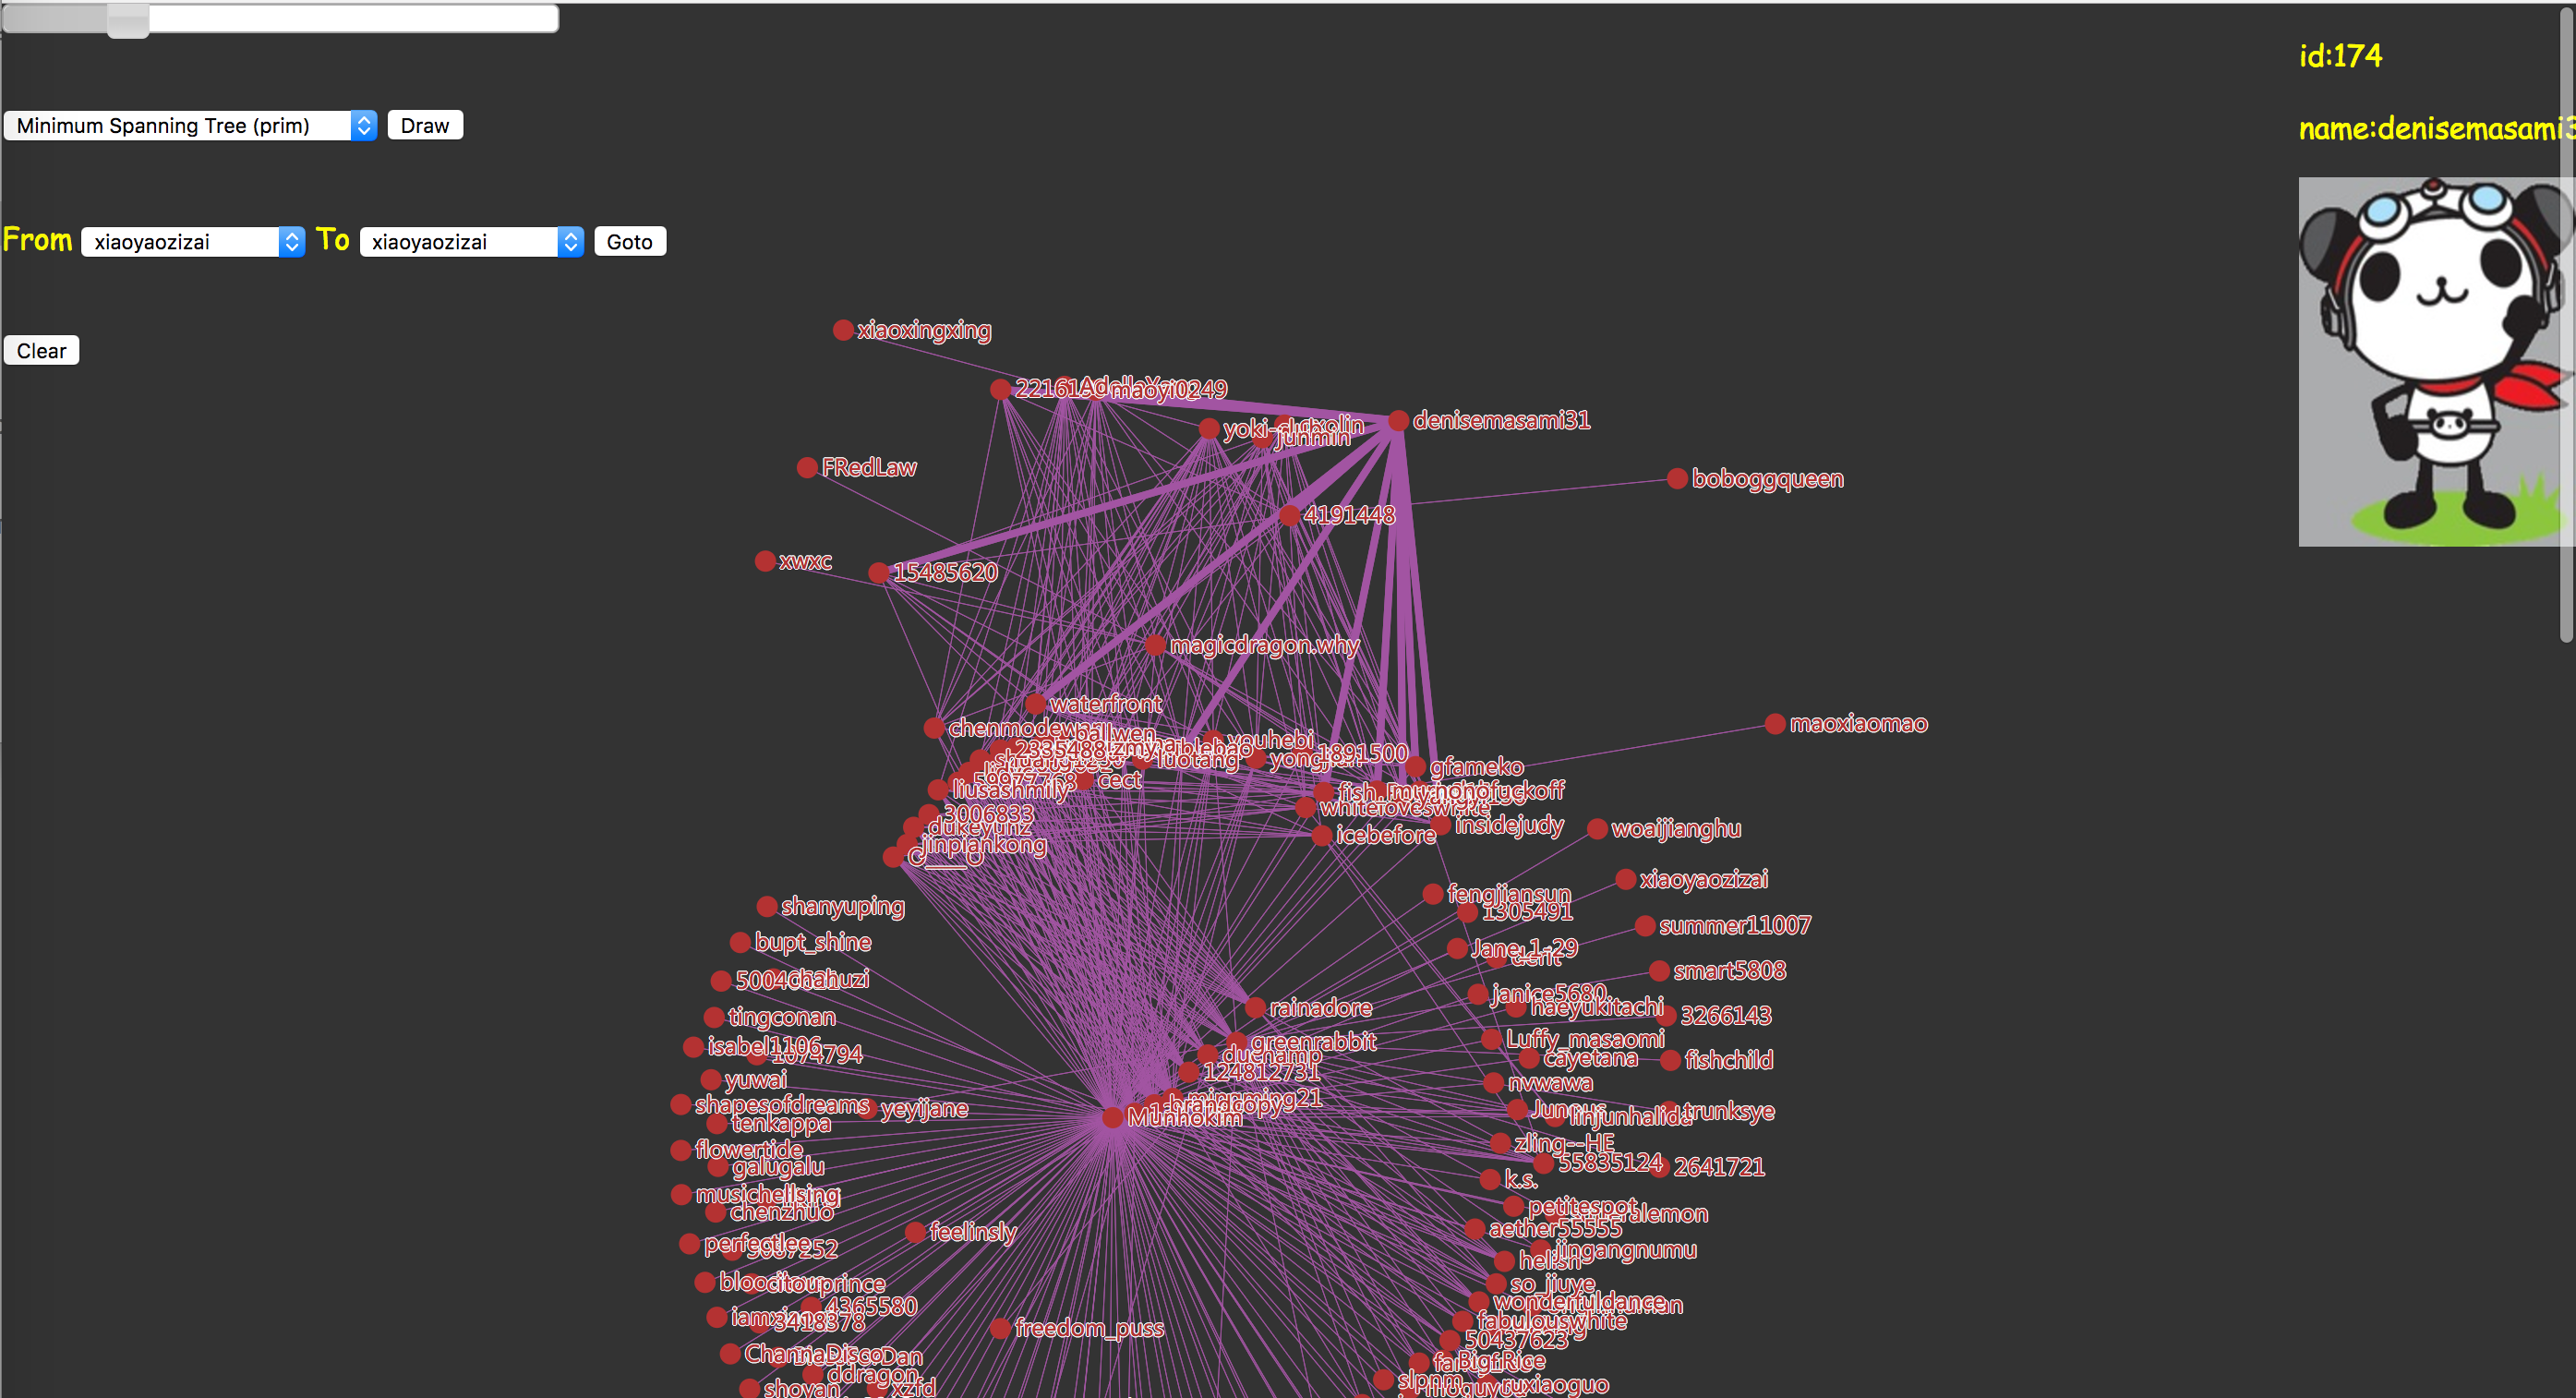
\includegraphics[width=1.0\columnwidth]{sample.png}
  \caption{Sample GUI.}
  \label{fig:sample}
\end{figure}
\subsection{Visualization}
After getting the processed data, we visualize data with D3 framework which is developed with Javascript programming language. From Figure~\ref{fig:sample}, we can see that every vertex of the graph is presented by a red circle and each edge is presented by a purple line. The characters near each vertex is its name. If you are interested in one vertex, you can click it and the detail of this vertex appears on the top right of the page including its id, name and icon. The tool bar is placed at the left top of the page, where each algorithm can be triggered when select the corresponding function. \\ 

\section{Algorithm}
\subsection{Basic Algorithm}
We implement all of the required basic algorithms: Prim Algorithm, Kruskal Algorithm, Dijkstra Algorithm, Ford Algorithm, Floyd Algorithm, Betweenness Centrality and Closeness Centrality. We choose to use JavaScript to implement all of the algorithm.
\subsubsection{Prim Algorithm}
Our goal is to find a minimum spanning tree for a weighted undirected graph by giving a starting vertex. This means we have to find a subset of the edges that forms a tree that includes every vertex, where the total weight of all the edges in the tree is minimized.\\
The algorithm operates by building this tree one vertex at a time, from the given starting vertex, at each step adding the cheapest possible connection from the tree to another vertex.
Detailed steps are as follows:\\\\
1. Initialize a tree with a single vertex, chosen by the user.\\\\
2. Grow the tree by one edge: of the edges that connect the tree to vertices not yet in the tree, find the minimum-weight edge, and transfer it to the tree.\\\\
3. Repeat step 2 (until all vertices are in the tree).\\\\
We use the adjacency list to represent the edges in the graph. Besides, in order to accelerate the choosen of the edge with minimal weight, we implement the PriorityQueue object by ourselves. The PriorityQueue use Fibonacci heap to accelerate the choosing process.
\subsubsection{Kruskal Algorithm}
Kruskal is a minimum spanning tree algorithm which finds the minimum spanning tree from edges of the graph. It first sorts all the edges of the graph according to their weight. Then it select the edge one by one in the sorted edge list and filter the edges whose two vertices are already connected in the current generated spanning tree. The algorithm's time complexity is $O(V logV)$. \\
In the implementation, the criterion that both vertices are connected now is hard to express. We observe that during the process of the algorithm, there are several sub spanning trees that will be connected by future edges. It's difficult to check whether two vertices on two sub spanning trees are both on the spanning tree. Thus, we only save the sub spanning tree id of each vertex and if two a edge has two vertices on two spanning trees, we regard these two trees as one tree and set a dict to map these two sub spanning tree id to one id (to the smaller id of these two). This can express the criterion more conveniently and speed up the algorithm. \\
\subsubsection{Dijkstra Algorithm}
Our goal is to find the shortest path between two choosen nodes. The steps of the algorithm is as follows:\\\\
1.Assign to every node a tentative distance value: set it to zero for our initial node and to infinity for all other nodes.\\\\
2.Set the initial node as current. Mark all other nodes unvisited. Create a set of all the unvisited nodes called the unvisited set.\\\\
3.For the current node, consider all of its unvisited neighbors and calculate their tentative distances. Compare the newly calculated tentative distance to the current assigned value and assign the smaller one. For example, if the current node A is marked with a distance of 6, and the edge connecting it with a neighbor B has length 2, then the distance to B (through A) will be 6 + 2 = 8. If B was previously marked with a distance greater than 8 then change it to 8. Otherwise, keep the current value.\\\\
4.When we are done considering all of the neighbors of the current node, mark the current node as visited and remove it from the unvisited set. A visited node will never be checked again.\\\\
5.If the destination node has been marked visited (when planning a route between two specific nodes) or if the smallest tentative distance among the nodes in the unvisited set is infinity (when planning a complete traversal; occurs when there is no connection between the initial node and remaining unvisited nodes), then stop. The algorithm has finished.\\\\
6.Otherwise, select the unvisited node that is marked with the smallest tentative distance, set it as the new "current node", and go back to step 3.\\\\
We also use adjacency list to represent the edges with weight in the graph. And we use Fibonacci heap to achieve the $O(E + VlogV)$ time complexity.
\subsubsection{Ford Algorithm}
Ford algorithm is shortest path algorithm which finds shortest path from on vertex to all the other vertices. This algorithm is a iterative algorithm and in every step, the shortest path of this step pass one more vertex than the previous step. And after at most $m$ steps, the algorithm will stop. Thus, the time complexity of this algorithm is $O(|V||E|)$.\\
In Ford algorithm, we only needs to save the current shortest path length and the directly pre-node of each vertex. And once no vertex's path is updated, the algorithm stops. In practice, we find that the algorithm usually needs less than $m$ steps.\\
\subsubsection{Floyd Algorithm}
Floyd algorithm finds all the shortest path between each two vertices. It updates the shortest path if the path will be closer when passing through another vertex. It has three nested loops and has a complexity of $O(n^3)$\\
This algorithm is useful when our graph is fixed during processing. Under this condition, we can calculate the shortest path only once and save the result. Every time the shortest path of two vertices is queried, the result can return the result directly, which speeds up average querying time. In practice, we use this idea and calculate the Floyd result once the user select "Floyd" and click "draw". Next time you set "from" and "to" the path will be returned directly. And if the data changes, the Floyd needs calculating carefully.\\
\subsubsection{Betweenness Centrality}
Betweenness centrality is a measure of centrality in a graph based on shortest paths. For every pair of vertices in a graph, there exists a shortest path between the vertices such that either the number of edges that the path passes through (for undirected graphs) or the sum of the weights of the edges (for directed graphs) is minimized. The betweenness centrality for each vertex is the number of these shortest paths that pass through the vertex. And our goal is to calculate the betweenness centrality for all of the nodes in the graph.$^{[2]}$
The betweenness centrality of a node \mbox{\boldmath $v$} is given by the expression:
\[g(v) = \sum_{s\neq v\neq t}\frac{\sigma_{st}(v)}{\sigma_{st}}\]
where \mbox{\boldmath $\sigma_{st}$} is the total number of shortest paths from node \mbox{\boldmath $s$} to node \mbox{\boldmath $t$} and \mbox{\boldmath $\sigma_{st}(v)$} is the number of those paths that pass through \mbox{\boldmath $v$}.
Note that the betweenness centrality of a node scales with the number of pairs of nodes as implied by the summation indices. Therefore, the calculation may be rescaled by dividing through by the number of pairs of nodes not including \mbox{\boldmath $v$}, so that \mbox{\boldmath $g \in [0,1]$}. The division is done by \mbox{\boldmath $(N - 1)(N - 2)/2$} for directed graphs and \mbox{\boldmath $(N - 1)(N - 2)/2$} for undirected graphs, where \mbox{\boldmath $N$} is the number of nodes in the giant component. Note that this scales for the highest possible value, where one node is crossed by every single shortest path. This is often not the case, and a normalization can be performed without a loss of precision
\[normal(g(v)) = \frac{g(v) - min(g)}{max(g) - min(g)}\]
which results in:
\[max(normal) = 1\]
\[min(normal) = 0\]
Note that this will always be a scaling from a smaller range into a larger range, so no precision is lost.\\
Calculating the betweenness centralities of all the vertices in a graph involves calculating the shortest paths between all pairs of vertices on a graph, which takes ${\displaystyle \Theta (|V|^{3})}$ time with the Floyd–Warshall algorithm, modified to not only find one but count all shortest paths between two nodes.\\
In calculating betweenness centralities of all vertices in a graph, it is assumed that graphs are undirected and connected with the allowance of loops and multiple edges. When specifically dealing with network graphs, often graphs are without loops or multiple edges to maintain simple relationships.\\
The betweenness of a vertex ${\displaystyle v}$ in a graph ${\displaystyle G:=(V,E)} $ with ${\displaystyle V}$ vertices is computed as follows:\\\\
1.For each pair of vertices (s,t), compute the shortest paths between them.\\\\
2.For each pair of vertices (s,t), determine the fraction of shortest paths that pass through the vertex in question (here, vertex v).\\\\
3.Sum this fraction over all pairs of vertices (s,t).\\\\
We use adjacency list to represent the edges, and in the algorithm we use queue and stack.
\subsubsection{Closeness Centrality}
In a connected graph, the closeness centrality of a node is a measure of centrality in a network, calculated as the sum of the length of the shortest paths between the node and all other nodes in the graph. Thus the more central a node is, the closer it is to all other nodes.\\
Closeness was defined as the reciprocal of the farness, that is:
\[C(x) = \frac{1}{\sum_{y}d(y, x)}\]
where $d(y, x)$ is the distance between vertices $x$ and $y$.\\
When a graph is not strongly connected, a widespread idea is that of using the sum of reciprocal of distances, instead of the reciprocal of the sum of distances, with the convention $1/\infty = 0$:
\[H(x) = \sum_{y\neq x}\frac{1}{d(y, x)}\]
In the classic definition of the closeness centrality, the spread of information is modeled by the use of shortest paths. This model might not be the most realistic for all types of communication scenarios. Thus, related definitions have been discussed to measure closeness.\\
Calculating the closeness centralities of all the vertices in a graph also involves calculating the shortest paths between all pairs of vertices on a graph.\\
In calculating closeness centralities of all vertices in a graph, it is assumed that graphs are undirected and connected with the allowance of loops and multiple edges. When specifically dealing with network graphs, often graphs are without loops or multiple edges to maintain simple relationships.\\
The steps of the algorithm are as follows:\\\\
1.Calculating the shortest paths between all pairs of vertices on a graph using Floyd–Warshall algorithm.\\\\
2.Calculate the closeness centralities based on the adjacency matrix.\\\\
3.Normalize the closeness by dividing the max centrality.\\\\
We use adjacency matrix to implement the Floyd-Warshall algorithm and post-processing.
\subsection{Advanced Algorithm}
\subsubsection{SLPA algorithm}
Community structure is considered to be a signnificant property of real-world social networks. In this project we implement an efficient algorithm for detecting both individual overlapping nodes and overlapping communities using the underlying network structure alone. This algorithm is called SLPA \cite{cite:SLPA}.\\
This algorithm is an extension of the Label Propagation Algorithm(LPA). In LPA, each node holds only a single label and iteratively updates it to its neighborhood majority label. This algorithm accounts for overlap by allowing each node to possess multiple labels but it uses different dynamics with more general features.\\
SLPA mimics human pairwise communication behavior. In each communication step, one node is a speaker(information provider), and the other is a listener(information consumer). Unlike other algorithms, each node has a $memory$ of the labels received in the past and takes its content into account to make the current decisions. This allows SLPA to avoid producing a number of small size communities as opposed to other algorithms.\\
The steps of this algorithm are as follows:\\\\
1.The $memory$ of each node is initialized with a unique label, in our project, we initialize it with the node's id.\\\\
2.The following steps are repeated until the maximum iteration $T$ is reached:\\\\
a. One node is selected as a listener. In our project we choose the node in the order of node's id.\\\\
b. Each neighbor of the selected node randomly selects a label with probability proportional to the occurrence frequency of this label in its memory and sends the selected label to the listener.\\\\
c. The listener adds the most popular label received to its memory.\\\\
3. The post-processing based on the labels in the memories and the threshold $r$ is applied to output the communities.\\\\
The algorithm explores the network and outputs the desired number of communities in the end. The size of memory increases by one for each node at each step. When $T$ is greater than 20, the algorithm produces stable outputs. Although SLPA is non-deterministic due to the random selection and ties, it performs well on average.\\
In SLPA, the detection of communities is performed when the stored information is post-processed. Given the memory of a node, SLPA converts it into a probability distribution of labels. Since labels represent community id, this distribution naturally defines the $strength$ of association to communities to which the node belongs. To preduce $crisp$ communities in which the membership of a node to a given community is binary, i.e., either a node is in a community or not, a simple thresholding procedure is performed: if the probability of seeing a particular label during the whole process is less than a given threshold $r \in [0, 0.5]$, this label is deleted. After thresholding, connected nodes having a particular label are grouped together and form a community. If a node contains multiple labels, it belongs to more than one community. A smaller value of $r$ produces a larger number of communities. When $r\geq 0.5$, SLPA outputs disjoint communities.\\
Noted that in our opinion, a single node can't be a community so we delete it.\\
We use adjacency list to represent the edges in the graph and store the $memory$ information in the node structure. Then we use a receiveList to choose the most popular node from the $Speaker$. Finally, we use a two-dimension array to store all of the communities.
\subsubsection{Information Flow}
In real life, the social network consists of nodes(users) and edges(relation) is always analysed to extract useful information form the network data. We select the event flow in real life and we want to mimic this process on the graph. We select one point as a start point and an event appears on this vertex, and simulate how the news of event will flow through the social network. This analysis finds the hidden structure of the social network and from the simulation, we can find some important vertices in the graph will block the information flow. Some vertices are transition vertices and these vertices receive much information from multiple vertices and send information to many vertices. If this vertex has some problems, the flow will be cut down. Based on these analyses, when events break up, the government or the corresponding authorization can control the flow immediately.\\
The function can be triggered, 
\section{Result}
  
\section{Conclusion}

\begin{small}
\bibliographystyle{unsrt}
\bibliography{document} 
\end{small}

\medskip

\end{document}
